%% Based on a TeXnicCenter-Template by Gyorgy SZEIDL.
%%%%%%%%%%%%%%%%%%%%%%%%%%%%%%%%%%%%%%%%%%%%%%%%%%%%%%%%%%%%%

%------------------------------------------------------------
%
\documentclass[10pt, a4paper]{article}%
%Options -- Point size:  10pt (default), 11pt, 12pt
%        -- Paper size:  letterpaper (default), a4paper, a5paper, b5paper
%                        legalpaper, executivepaper
%        -- Orientation  (portrait is the default)
%                        landscape
%        -- Print size:  oneside (default), twoside
%        -- Quality      final(default), draft
%        -- Title page   notitlepage, titlepage(default)
%        -- Columns      onecolumn(default), twocolumn
%        -- Equation numbering (equation numbers on the right is the default)
%                        leqno
%        -- Displayed equations (centered is the default)
%                        fleqn (equations start at the same distance from the right side)
%        -- Open bibliography style (closed is the default)
%                        openbib
% For instance the command
%           \documentclass[a4paper,12pt,leqno]{article}
% ensures that the paper size is a4, the fonts are typeset at the size 12p
% and the equation numbers are on the left side
%
\usepackage{amsmath}%
\usepackage{amsfonts}%
\usepackage{amssymb}%
\usepackage{graphicx}
\usepackage{polski}
\usepackage[UTF8]{inputenc}
\usepackage{enumerate}
\usepackage{pdflscape}
\usepackage{wrapfig}
\usepackage[a4paper, left=2.5cm, right=2.5cm, top=3.5cm, bottom=3.5cm, headsep=1.2cm]{geometry}
%-------------------------------------------
\newtheorem{theorem}{Theorem}
\newtheorem{acknowledgement}[theorem]{Acknowledgement}
\newtheorem{algorithm}[theorem]{Algorithm}
\newtheorem{axiom}[theorem]{Axiom}
\newtheorem{case}[theorem]{Case}
\newtheorem{claim}[theorem]{Claim}
\newtheorem{conclusion}[theorem]{Conclusion}
\newtheorem{condition}[theorem]{Condition}
\newtheorem{conjecture}[theorem]{Conjecture}
\newtheorem{corollary}[theorem]{Corollary}
\newtheorem{criterion}[theorem]{Criterion}
\newtheorem{definition}[theorem]{Definition}
\newtheorem{example}[theorem]{Example}
\newtheorem{exercise}[theorem]{Exercise}
\newtheorem{lemma}[theorem]{Lemma}
\newtheorem{notation}[theorem]{Notation}
\newtheorem{problem}[theorem]{Problem}
\newtheorem{proposition}[theorem]{Proposition}
\newtheorem{remark}[theorem]{Remark}
\newtheorem{solution}[theorem]{Solution}
\newtheorem{summary}[theorem]{Summary}
\newenvironment{proof}[1][Proof]{\textbf{#1.} }{\ \rule{0.5em}{0.5em}}

\begin{document}

\title{Opis Projektu}
\author{Paweł Warzecha}
\date{2 marca 2016}
\maketitle

\section{Opis ogólny}

\hspace{15pt}Przedmiotem projektu jest budowa działa laserowego wyposażonego w system wizyjny umożliwiający rozpoznawanie celów. Tego typu urządzenia są budowane do zabijania komarów w Afryce co ma zredukować ilość zachorowań na malarie. Jednak taki system ma znacznie większy potencjał, dlatego nasz projekt zostanie zbudowany w pełni w oparciu o oprogramowanie na licencji Open Source oraz będzie rozpowszechniany na jej zasadach. W ten sposób każdy będzie mógł dokonać modyfikacji aby dopasować projekt do swoich potrzeb. Spodziewanym efektem prac będzie działo laserowe z dwoma trybami pracy, automatycznym i ręcznym. Sterowanie ręczne będzie odbywało przy pomocy kontrolera podłączonego do komputera zewnętrznego, który będzie komunikował się z komputerem pokładowym przez sieć WI-FI. Projekt ma za zadanie opracowania metod komunikacji między dwoma systemami opartymi na różnej architekturze procesora oraz opracowanie algorytmów przetwarzania obrazu. Wyniki prac będą zamieszczanie na stronie www pod adresem
http://89.72.70.224/laser.html.



\section{Plan prac i rozkład obowiązków}

\noindent \newline Kamienie milowe: 

\begin{itemize}
  \item Działający algorytm przetwarzania obrazu
  \item Działająca komunikacja
	\item Ukończony interfejs użytkownika
\end{itemize}

\begin{landscape}
\begin{figure}[h]
\begin{center}

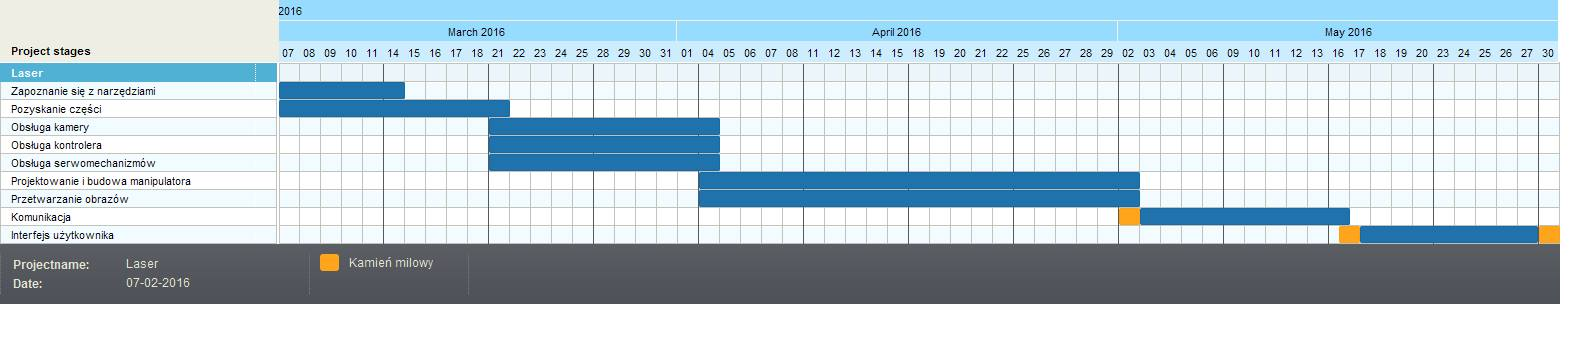
\includegraphics[width=1.25\textwidth,height = 0.5\textwidth]{gantt3}
\caption{Wykres Gantta}
\end{center}
\end{figure}
\end{landscape}




\newpage


\section{Doręczenie}

\begin{tabular}{|c|c|c|} \hline
	
	Data & Nazwa & Postać\\
	\hline
  2.05.2016 & Działo autonomiczne & Oprogramowanie i dokumentacja \\
	\hline
	16.05.2016 & Sterowanie ręczne & Oprogramowanie i dokumentacja\\
	\hline
	30.05.2016 & Interfejs użytkownika & Oprogramowanie i dokumentacja \\
	\hline
	6.06.2016 &  Raport końcowy & Raport końcowy\\
	\hline
\end{tabular}

\section{Budżet}

\begin{tabular}{|r|l|} \hline

  Laser 5000mW & 60 zł \\
  Serwo mechanizmy & 20 zł \\
	Plexa & 20 zł\\
	Tranzystor MOSFET & 2 zł \\
	Balony & 10 zł \\
  \hline
  Łącznie & 112 zł \\
  \hline

\end{tabular}

\section{Zarządzanie projektem}
\hspace{15pt}Każdy członek zespołu zobowiązany jest pracować na dysku zdalnym udostępnianym przez kierownika projektu, dzięki temu kierownik będzie miał pełny wgląd w postęp prac i będzie mógł na bieżąco zgłaszać uwagi. Komunikacja będzie odbywała się na prywatnej grupie w serwisie facebook.com. Każdy członek jest zobowiązany do stworzenia dokumentacji z części projektu którą stworzył, a kierownik do złożenia poszczególnych części w całość. W razie wystąpienia konfliktu i niemożności rozstrzygnięcia go w gronie osób skonfliktowanych, problem zostanie omówiony na forum zespołu w specjalnie do tego wyznaczonym terminie. Okresowe spotkania w celu omówienia postępu prac będą odbywały się pod koniec każdego miesiąca.
\section{Zespół}

Paweł Warzecha - koordynator projektu\\
Kacper Pawlak - obsługa kamery i algorytm przetwarzania obrazu\\
Bartosz Kowalski - obsługa kamery i algorytm przetwarzania obrazu\\
Jacek Kamienicki - algorytm sterowania serwomechanizmami\\
Adam Burdykiewicz - obsługa kontrolera i projekt manipulatora\\
Kamil Orłow - interfejs użytkownika\\
Piotr Bachry - komunikacja\\

\end{document}
